% -*- coding: utf-8 -*-
\section{Introduction}
The field of plasmonics which explores the interaction of light with metals has gained tremendous interest over the past few years \cite{ozbay_plasmonics:_2006}. Several numerical techniques have been proposed to study the interaction/propagation of electromagnetic waves with metals \cite{smajic_comparison_2009}, and one of the most popular and widely accepted techniques is the finite-difference time-domain (FDTD) method \cite{taflove_computational_2005}. FDTD being a time domain technique, offers several advantages particularly for the study of light-metal interaction since the frequency response of the system under study over a wide range of frequencies can be obtained with a single run of simulation.

The frequency-dependent electric permittivity is an important parameter to be known in advance when studying the frequency response of the material over a wide frequency range. Traditionally, Drude-Lorentz (DL\index{DL model}) model\index{Drude-Lorentz model} which can well represent the optical properties of the metal originating from the interband and intraband transitions was the popular one and has been used to quantify the dispersion properties of the metal. In DL model, a large number of Lorentz oscillators can be used to model the line shape of the electric permittivity of the material over the frequency range of interest \cite{etchegoin_analytic_2006}. However, the accuracy improvement obtained via adding more Lorentz terms comes with a price. A large number of Lorentz terms\index{Lorentz term} lead to increased requirement of computational resources such as CPU power and memory \cite{young_summary_2001}. 

Recently, Drude-critical point (DCP\index{DCP model}) model\index{Drude-critical point model} that consists of one Drude term and two critical point terms was proposed which can satisfactorily represent the electric permittivity of metals over a wide frequency range \cite{etchegoin_analytic_2006, etchegoin_erratum:_2007}. From the computational perspective, DCP model\index{DCP model} is advantageous over DL model\index{DL model} since the former requires only less number of terms. Since then, DCP model\index{DCP model} has been used to represent the electric permittivity of metals such as gold and others with good accuracy \cite{vial_comparison_2008}. 

Several implementation techniques are available to model dispersive media in the FDTD\index{FDTD} algorithm. For example, \citet{kelley_piecewise_1996} proposed a piecewise-linear recursive-convolution (PLRC\index{PLRC method}) method\index{piecewise-linear recursive-convolution method} to implement the Debye and Lorentz dispersive media and the results were compared to that of \citet{luebbers_fdtd_1993} which used the RC method. \citet{vial_implementation_2007} implemented the DCP model\index{DCP model} by using RC method\index{RC method} while \citet{sullivan_electromagnetic_2000, weedon_general_1997} used the Z-transform technique\index{Z-transform technique} to implement dispersive media into the FDTD\index{FDTD} algorithm. An ADE technique\index{ADE method} to implement the Lorentz dispersive model was proposed \cite{joseph_direct_1991} and it was shown by \citet{okoniewski_simple_1997} that the usage of the ADE scheme resulted in reduced computational burden compared to that of PLRC technique. 

In this work, we will show the FDTD\index{FDTD} implementation of DCP dispersive model by using two popular techniques, i.e. PLRC and ADE. Memory requirements as well as the accuracy for each implementations are analyzed in detail. Numerical results are compared to that of analytical results for the case of reflection and transmission of light through thin metal films in order to validate the proposed implementation schemes.  

\section{FDTD implementation}
\label{sec:d2cp}
The DCP dispersive model\index{DCP model} expresses interband transitions featuring asymmetric line shapes with critical point terms instead of Lorentzian terms\index{Lorentzian term} \cite{etchegoin_analytic_2006}. The relative electric permittivity as per the DCP model\index{DCP model} can be written as
\begin{equation}
\epsilon_r(\omega) = \epsilon_\infty + \chi_D(\omega) + \sum_{p=1}^2 \chi_p(\omega)
\label{eq:dcp}
\end{equation}
where $\epsilon_\infty$ is the relative electric permittivity at infinite frequency, $\chi_D(\omega)$ is the Drude susceptibility\index{Drude susceptibility}, and $\chi_p(\omega)$ is the critical point susceptibility. The Drude susceptibility\index{Drude susceptibility} is expressed as
\begin{equation}
\chi_D(\omega) = - \frac{\omega_D^2}{\omega^2 + i \gamma \omega}
\label{eq:drude}
\end{equation}
where $\omega_D$ is the Drude pole frequency, and $\gamma$ is the inverse of the pole relaxation time. Also, the critical point susceptibility is expressed as
\begin{equation}
\chi_p(\omega) = A_p \Omega_p \left ( \frac{e^{i\phi_p}}{\Omega_p - \omega -i \Gamma_p} + \frac{e^{-i \phi_p}}{\Omega_p + \omega + i \Gamma_p} \right )
\label{eq:cp}
\end{equation}
where $A_p$ is the amplitude, $\phi_p$ is the phase, $\hbar\Omega_p$ is the energy gap, and $\Gamma_p$ is the broadening of the pole. The time dependence is described following the $e^{-i \omega t}$ convention. In the following, PLRC and ADE implementation of the DCP model is shown.

\subsection{Numerical implementation in PLRC}
\label{sec:impl_plrc}
The PLRC method uses a linear approximation to evaluate the electric field $\mathbf{E}(t)$ over each time-stepping interval \cite{kelley_piecewise_1996} and has better accuracy compared to the RC method which assumes a constant electric field over the time-stepping interval. The equation for updating the electric field $\mathbf{E}^{n}$ at time-step $t=n\Delta t$ is
\begin{equation}
\begin{split}
\mathbf{E}^{n+1} = & ~ \frac{2 \Delta t}{2 \epsilon_0 \left( \epsilon_\infty - \xi^0 + \chi^0 \right) + \sigma \Delta t} \nabla \times \mathbf{H}^{n+1/2}\\
& + \frac{2 \epsilon_0 \left( \epsilon_\infty - \xi^0 \right) - \sigma \Delta t}{2 \epsilon_0 \left( \epsilon_\infty - \xi^0 + \chi^0 \right) + \sigma \Delta t} \mathbf{E}^n\\
& + \frac{2 \epsilon_0}{2 \epsilon_0 \left( \epsilon_\infty - \xi^0 + \chi^0 \right) + \sigma \Delta t} \mathbf{\Psi}^n
\end{split}
\label{eq:plrc_update_e}
\end{equation}
where
\begin{equation}
\begin{split}
\chi^0 = & ~ \chi_D^0 + \Re \left ( \sum_p \hat \chi_p^0 \right)\\
\xi^0 = & ~ \xi_D^0 + \Re \left ( \sum_p \hat \xi_p^0 \right )\\
\mathbf \Psi^n = & ~ \mathbf \Psi_D^n + \Re \left ( \sum_p \hat{\mathbf \Psi}_p^n \right ).
\label{eq:plrc_sums}
\end{split}
\end{equation}

The exact forms of the variables on the right hand side of Eq.~(\ref{eq:plrc_sums}) are described in sections \ref{sec:plrc_dp} and \ref{sec:plrc_cp}. $\mathbf{\Psi}^n$ is the recursive accumulator which is the convolutional sum of electric field and temporal susceptibility. $\sigma$ is the electrical conductivity, $\epsilon_0$ is the vacuum permittivity, and $\Delta t$ is the time-stepping interval. The ``$\hat{~~}$'' denotes a complex number. If we set $\xi_D^0$, $\hat \xi_D^0$, $\Delta \xi_D^0$, and $\Delta \hat \xi_D^0$ to 0, then Eqs.~(\ref{eq:plrc_update_e}, \ref{eq:plrc_sums}, \ref{eq:rec_accu_dp}, \ref{eq:rec_accu_cp}) become identical to that of RC implementation in \citet{vial_implementation_2007}.

\subsubsection{The Drude term}
\label{sec:plrc_dp}
The time-domain susceptibility function $\chi_D(t)$ is obtained by inverse Fourier transformation of Eq.~(\ref{eq:drude}), yielding
\begin{equation}
\chi_D(t) = \frac{\omega_D^2}{\gamma} (1 - e^{-\gamma t}) U(t)
\label{eq:drude_t}
\end{equation}
where $U(t)$ is the unit step function. Substituting Eq.~(\ref{eq:drude_t}) into the definition of $\chi^m$ and $\xi^m$ shown in \citet{kelley_piecewise_1996}, we obtain the following equations
\begin{equation}
\begin{split}
&\chi_D^0 = \frac{\omega_D^2}{\gamma^2} (e^{-\gamma \Delta t} + \gamma \Delta t - 1)\\
&\xi_D^0 = \chi_D^0 \left ( \frac{1}{1 - e^{\gamma \Delta t}} + \frac{1}{\gamma \Delta t} \right ) - \frac{\omega_D^2}{\gamma^2} \left ( 1 - \frac{\gamma \Delta t}{2} \coth \frac{\gamma \Delta t}{2} \right )
\end{split}
\end{equation}
which are used for updating the electric field. The coefficients that are necessary for the recursive accumulator of the Drude pole are given by
\begin{equation}
\begin{split}
& \Delta \chi_D^0 = - \frac{\omega_D^2}{\gamma^2} (1 - e^{-\gamma \Delta t})^2\\
& \Delta \xi_D^0 = \Delta \chi_D^0 \left ( \frac{1}{1 - e^{\gamma \Delta t}}  + \frac{1}{\gamma \Delta t} \right ).
\end{split}
\end{equation}
Also, the recursive accumulator $\mathbf{\Psi}_D^n$ for the Drude pole obeys the following recursion relation
\begin{equation}
\mathbf{\Psi}_D^{n+1} = (\Delta\chi_D^0 - \Delta\xi_D^0) \mathbf{E}^{n+1} + \Delta \xi_D^0 \mathbf{E}^n + e^{-\gamma \Delta t} \mathbf{\Psi}_D^n.
\label{eq:rec_accu_dp}
\end{equation}

\subsubsection{Critical point terms}
\label{sec:plrc_cp}
The time-domain susceptibility function $\chi_p(t)$ is obtained by inverse Fourier transformation of Eq.~(\ref{eq:cp}), and is written as
\begin{equation}
\chi_p(t) = 2 A_p \Omega_p e^{-\Gamma_p t} \sin(\Omega_p t- \phi_p) U(t).
\label{eq:cp_t}
\end{equation}
$\chi_p(t)$ has the form similar to the real-valued time-domain susceptibility function for the case of Lorentzian media and does not lead to a simple recursion relation for $\chi^m$ and $\xi^m$ \cite{kelley_piecewise_1996}. Hence we need to define a new complex-valued quasi-time-domain function \cite{vial_implementation_2007}
\begin{equation}
\hat{\chi}_p(t) = 2 i A_p \Omega_p e^{-\Gamma_p t - i (\Omega_p t - \phi_p)} U(t).
\end{equation}
The form of $\hat{\chi}_p(t)$ is close to that for the Lorentzian case \cite{kelley_piecewise_1996}, thus the procedure detailed in the case of a combination of Drude and Lorentzian terms can be applied, and steps required for the numerical implementation of the critical point model can be derived similar to \citet{vial_description_2007}. Substituting $\hat{\chi}_p(t)$ for $\chi(t)$ in the definition of $\chi^m$ and $\xi^m$, we obtain
\begin{equation}
\begin{split}
&\hat{\chi}_p^0 = \frac{2 i A_p \Omega_p e^{i \phi_p} (1 - e^{-\Delta t(\Gamma_p + i \Omega_p)})}{\Gamma_p + i \Omega_p}\\
&\hat{\xi}_p^0 = \hat{\chi}_p^0 \left ( \frac{1}{1 - e^{\Delta t (\Gamma_p + i \Omega_p)}} + \frac{1}{\Delta t (\Gamma_p + i \Omega_p)} \right )
\end{split}
\end{equation}
for updating the electric field. The recursive accumulator for the critical point term becomes complex as in the case of Lorentz media. The recursion relation for the recursive accumulator of the $p$th critical point is written as
\begin{equation}
\hat{\mathbf{\Psi}}_p^{n+1} = (\Delta \hat \chi_p^0 - \Delta \hat \xi_p^0) \mathbf{E}^{n+1} + \Delta \hat \xi_p^0 \mathbf{E}^n + e^{-\Delta t (\Gamma_p + i \Omega_p)} \hat{\mathbf{\Psi}}_p^n
\label{eq:rec_accu_cp}
\end{equation}
with the following parameters
\begin{equation}
\begin{split}
&\Delta \hat \chi_p^0 = \frac{2 i A_p \Omega_p e^{i \phi_p} (1 - e^{- \Delta t (\Gamma_p + i \Omega_p)})^2}{\Gamma_p + i \Omega_p}\\
&\Delta \hat \xi_p^0 = \Delta \hat \chi_p^0 \left ( \frac{1}{1 - e^{\Delta t (\Gamma_p + i \Omega_p)}} + \frac{1}{\Delta t (\Gamma_p + i \Omega_p)} \right ).
\end{split}
\end{equation}

Thus, the PLRC scheme for modeling a DCP dispersive medium in the FDTD algorithm is essentially a four-step explicit procedure, and can be briefed as follows: Starting with the known values of $\mathbf{E}^{n}$, $\mathbf{\Psi}_D^n$, $\hat{\mathbf\Psi}_p^n$, $\mathbf{H}^{n+1/2}$, we first calculate $\mathbf{\Psi}^n$ using the last equation of Eq.~(\ref{eq:plrc_sums}) and then calculate $\mathbf{E}^{n+1}$ which is the updated electric field using Eq.~(\ref{eq:plrc_update_e}). With the updated electric field, we can then update recursive accumulators for each poles using Eq.~(\ref{eq:rec_accu_dp}) and (\ref{eq:rec_accu_cp}). Finally, $\mathbf{H}^{n+3/2}$ is obtained from $\mathbf{H}^{n+1/2}$ and $\mathbf{E}^{n+1}$ in the usual manner from the Yee realization of Faraday's law, and this cycle repeats for every time-step.

\subsection{Numerical implementation in ADE}
The ADE scheme is simpler than the PLRC scheme. Using the complex phasor notation, the differential form of Ampere's law can be expressed for a DCP medium as
\begin{equation}
\nabla \times \breve{\mathbf H} = -i \epsilon_0 \epsilon_\infty \omega \breve{\mathbf E} - i \omega \breve{\mathbf P}_D - i \omega \sum_p \breve {\mathbf P}_p + \sigma \breve{\mathbf E}
\label{eq:amperes_law}
\end{equation}
where $\breve{\mathbf P}_D$ and $\breve{\mathbf P}_p$ are the polarization fields represented in the form of
\begin{equation}
\breve{\mathbf P}_D = \epsilon_0 \chi_D(\omega) \breve{\mathbf E}
\label{eq:dispersion_current_dp}
\end{equation}
and
\begin{equation}
\breve{\mathbf P}_p = \epsilon_0 \chi_p(\omega) \breve{\mathbf E}.
\label{eq:dispersion_current_cp}
\end{equation}
Here, ``$\breve{~~}$'' denotes the quantity in frequency domain. The inverse Fourier transformation of Eq.~(\ref{eq:amperes_law}) can be implemented in FDTD at a fixed time $(n + 1/2) \Delta t$ using the central differencing and semi-implicit scheme, where yet-to-be-computed fields at time-step $n+1$ are used to create an update formula for a field known at time-step $n$ given by
\begin{equation}
\begin{split}
\mathbf{E}^{n+1} =& ~ \frac{2 \Delta t}{2 \epsilon_0 \epsilon_\infty + \sigma \Delta t} \nabla \times \mathbf{H}^{n+1/2}\\
& - \frac{2 \left ( \mathbf{P}_D^{n+1}- \mathbf{P}_D^n \right)}{2 \epsilon_0 \epsilon_\infty + \sigma \Delta t} - \frac{2 \sum_p \left( \mathbf{P}_p^{n+1} - \mathbf{P}_p^n \right)}{2 \epsilon_0 \epsilon_\infty + \sigma \Delta t}\\
& + \frac{2 \epsilon_0 \epsilon_\infty - \sigma \Delta t}{2 \epsilon_0 \epsilon_\infty + \sigma \Delta t} \mathbf{E}^n.
\label{eq:e_update_ade_tmp}
\end{split}
\end{equation}
This equation cannot be used to update electric field yet, since the right hand side of it contains yet-to-be-computed values of $\mathbf{P}_D^{n+1}$, $\mathbf{P}_p^{n+1}$. Thus we require auxiliary equations to compute those variables.

\subsubsection{The Drude term}
\label{sec:ade_dp}
The Drude term can be converted into a form suitable to be used in the time-stepping scheme by using the method introduced by \citet{okoniewski_drude_2006} without losing the second-order nature of the model. By applying the central differencing and semi-implicit scheme at $n$ on the inverse Fourier transformation of Eq.~(\ref{eq:dispersion_current_dp}), we get the equation for the Drude field at the time-step $n+1$ as
\begin{equation}
\mathbf{P}_D^{n+1} = a_0 \mathbf{P}_D^{n-1} + a_1 \mathbf{P}_D^n + a_2 \left( \mathbf{E}^{n-1} + 2 \mathbf{E}^n + \mathbf{E}^{n+1} \right)
\label{eq:dispersion_current_dp_n}
\end{equation}
where 
\begin{equation}
\begin{split}
&a_0 = \frac{\gamma \Delta t - 2}{\gamma \Delta t + 2}\\
&a_1 = \frac{4}{\gamma \Delta t + 2}\\
&a_2 = \frac{\Delta t^2 \epsilon_0 \omega_D^2}{2 (\gamma \Delta t + 2)}.
\end{split}
\end{equation}

\subsubsection{Critical point terms}
\label{sec:ade_cp}
By applying the central difference scheme at $n$ on the inverse Fourier transformation of Eq.~(\ref{eq:dispersion_current_cp}), we obtain the equation for critical point terms at time-step $n+1$ as
\begin{equation}
\mathbf{P}_p^{n+1} = b_{p,0} \mathbf{P}_p^{n-1} + b_{p,1} \mathbf{P}_p^n + b_{p,2} \mathbf{E}^{n-1} +  b_{p,3} \mathbf{E}^{n} + b_{p,4} \mathbf{E}^{n+1}
\label{eq:dispersion_current_cp_n}
\end{equation}
where
\begin{equation}
\begin{split}
&b_{p,0} = - \frac{\Omega_p^2 \Delta t^2 + (2 - \Gamma_p \Delta t)^2}{\Omega_p^2 \Delta t^2 + (2 + \Gamma_p \Delta t)^2}\\
&b_{p,1} = 2 \frac{4 - (\Gamma_p^2 + \Omega_p^2) \Delta t^2}{\Omega_p^2 \Delta t^2 + (2 + \Gamma_p \Delta t)^2}\\
&b_{p,2} = 2 \epsilon_0 A_p \Omega_p \Delta t \frac{\Omega_p \Delta t \cos \phi_p + (2 - \Gamma_p \Delta t) \sin \phi_p}{\Omega_p^2 \Delta t^2 + (2 + \Gamma_p \Delta t)^2}\\
&b_{p,3} = 4 \epsilon_0 A_p \Omega_p \Delta t \frac{\Omega_p \Delta t \cos \phi_p - \Gamma_p \Delta t \sin \phi_p}{\Omega_p^2 \Delta t^2 + (2 + \Gamma_p \Delta t)^2}\\
&b_{p,4} = 2 \epsilon_0 A_p \Omega_p \Delta t \frac{\Omega_p \Delta t \cos \phi_p - (2 + \Gamma_p \Delta t) \sin \phi_p}{\Omega_p^2 \Delta t^2 + (2 + \Gamma_p \Delta t)^2}.
\end{split}
\end{equation}

Substituting Eqs.~(\ref{eq:dispersion_current_dp_n}, \ref{eq:dispersion_current_cp_n}) into Eq.~(\ref{eq:e_update_ade_tmp}) and with few algebraic manipulation, we obtain the following explicit time-stepping relation for $\mathbf{E}$:
\begin{equation}
\begin{split}
\mathbf{E}^{n+1} = & ~ c_0 \nabla \times \mathbf{H}^{n+1/2}\\
& + c_1 \left( - a_0 \mathbf{P}_D^{n-1} + (1 - a_1) \mathbf{P}_D^n \right)\\
& + c_1 \sum_p \left( - b_{p,0} \mathbf{P}_p^{n-1} + (1 - b_{p,1}) \mathbf{P}_p^n \right)\\
& + c_2 \mathbf{E}^{n-1} + c_3 \mathbf{E}^n
\end{split}
\label{eq:e_update_ade_final}
\end{equation}
where
\begin{equation}
\begin{split}
&c_0 = \frac{\Delta t}{\sigma \Delta t / 2 + a_2 + \sum_p b_{p,4} + \epsilon_0 \epsilon_\infty}\\
&c_1 = \frac{1}{\sigma \Delta t / 2 + a_2 + \sum_p b_{p,4} + \epsilon_0 \epsilon_\infty}\\
&c_2 = - \frac{a_2 + \sum_p b_{p,2}}{\sigma \Delta t / 2 + a_2 + \sum_p b_{p,4} + \epsilon_0 \epsilon_\infty}\\
&c_3 = - \frac{\sigma \Delta t / 2 + 2 a_2 + \sum_p b_{p,3} - \epsilon_0 \epsilon_\infty}{\sigma \Delta t / 2 + a_2 + \sum_p b_{p,4} + \epsilon_0 \epsilon_\infty}.
\end{split}
\end{equation}

The ADE scheme for modeling a DCP dispersive medium in the FDTD algorithm is a three-step fully explicit procedure. Starting with the known values of $\mathbf{E}^{n-1}$, $\mathbf{E}^n$, $\mathbf{P}_D^{n-1}$, $\mathbf{P}_D^n$, $\mathbf{P}_p^{n-1}$, $\mathbf{P}_p^n$, and $\mathbf{H}^{n+1/2}$, we first calculate $\mathbf{E}^{n+1}$ using Eq.~(\ref{eq:e_update_ade_final}). Second, we calculate $\mathbf{P}_D^{n+1}$ and $\mathbf{P}_p^{n+1}$ using Eqs.~(\ref{eq:dispersion_current_dp_n}) and (\ref{eq:dispersion_current_cp_n}), respectively, along with the value of $\mathbf{E}^{n+1}$ that was just computed. Finally, $\mathbf{H}^{n+3/2}$ is obtained from $\mathbf{H}^{n+1/2}$ and $\mathbf{E}^{n+1}$ in the usual manner from the Yee realization of Faraday's law, and this cycle repeats for every FDTD time-step. Note that in contrast with the PLRC scheme, the ADE implementation uses only real parameters, and hence it can be used for updating complex electromagnetic field as well by just changing the type of field variables.

\section{Memory usage}
Figures \ref{fig:plrc_memory} and \ref{fig:ade_memory}, respectively, show the schematic flowcharts which describes the components used for PLRC and ADE implementations between two successive time-marching steps. In calculating Drude as well as critical point terms, the PLRC implementation requires a smaller number of components and about 22 \% less memory than ADE. 

The ADE method, however, has an advantage of requiring relatively fewer arithmetic operations to the PLRC method as shown in figures where the number of arrows, which represent arithmetic operations in figure \ref{fig:ade_memory} is fewer than shown in figure \ref{fig:plrc_memory}. It can also be implemented more efficiently than the PLRC method since the schematic flows for Drude and critical point terms in the ADE scheme are identical to each other and have fewer number of steps compared to the PLRC scheme as shown in figure \ref{fig:ade_memory}. This is another advantage of the ADE method over the PLRC method.
\begin{figure}[hp!]
  \begin{center}
    \subfigure[]{
      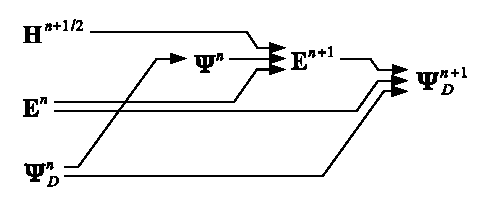
\includegraphics{figure/plrc_dp}
      \label{fig:plrc_dp}
    }
    \subfigure[]{
      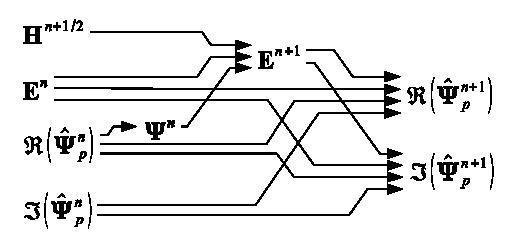
\includegraphics{figure/plrc_cp}
      \label{fig:plrc_cp}
    }
  \end{center}
  \caption{Schematic flowcharts for (a) a Drude term and (b) a critical point term for the PLRC implementation of DCP model}
  \label{fig:plrc_memory}
\end{figure}

\begin{figure}[hp!]
  \begin{center}
    \subfigure[]{
      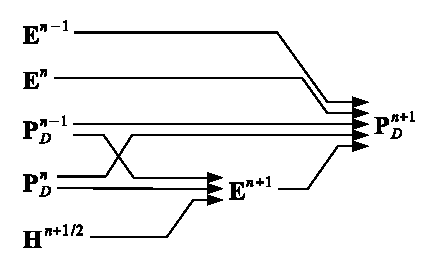
\includegraphics{figure/ade_dp}
      \label{fig:ade_dp}
    }
    \subfigure[]{
      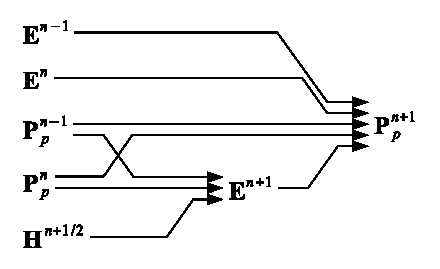
\includegraphics{figure/ade_cp}
      \label{fig:ade_cp}
    }
  \end{center}
  \caption{Schematic flowcharts for (a) a Drude term and (b) a critical point term for the ADE implementation of DCP model}
  \label{fig:ade_memory}
\end{figure}

\section{Accuracy estimates}
We can determine the accuracy\index{accuracy} of each implementation schemes using the generalized time-sampled relation ship between polarization and electric fields \cite{hulse_dispersive_1994, lin_accuracy_2009} given by
\begin{equation}
g_0 \mathbf{P}^{n-1} + g_1 \mathbf{P}^n + g_2 \mathbf{P}^{n+1} = \epsilon_0 \left(h_0 \mathbf{E}^{n-1} + h_1 \mathbf{E}^n + h_2 \mathbf{E}^{n+1} \right).
\label{eq:time_sampled_form}
\end{equation}
Substituting the time harmonic solutions $\mathbf{P}^n = \mathbf{P}_0 e^{-i \omega n \Delta t}$, $\mathbf{E}^n = \mathbf{E}_0 e^{-i \omega n \Delta t}$ into Eq.~(\ref{eq:time_sampled_form}), we get the numerical susceptibility as
\begin{equation}
\begin{split}
\tilde{\chi}(\omega) = &~ \frac{P(\omega)}{\epsilon_0 E(\omega)}\\
= &~ \frac{e^{i \Delta t \omega} h_0 + h_1 + e^{-i \Delta t \omega} h_2}{e^{i \Delta t \omega} g_0 + g_1 + e^{-i \Delta t \omega} g_2}\\
\end{split}
\end{equation}
where ``$\tilde{~~}$'' indicates the numerical representation of the quantity.

\subsection{Numerical susceptibility of PLRC implementation}
In the PLRC scheme, the polarization field at a time-step $n$ is expressed as \cite{kelley_piecewise_1996} 
\begin{equation}
\mathbf{P}^n = \epsilon_0 \sum_{m=0}^{n-1} \left ( \mathbf{E}^{n-m} \chi^m + \left ( \mathbf{E}^{n-m-1} - \mathbf{E}^{n-m} \right ) \xi^m \right ).
\label{eq:plrc_p_field}
\end{equation}
By converting  Eq.~(\ref{eq:plrc_p_field}) to the form of Eq.~(\ref{eq:time_sampled_form}) and by comparing the coefficients, we get
\begin{equation}
\begin{split}
& g_1 = \frac{\xi^m \chi^{m-2} - \xi^{m-2} \chi^m}{\xi^{m-1} \chi^m - \xi^m \chi^{m-1}} g_0\\
& g_2 = \frac{\xi^{m-2} \chi^{m-1} - \xi^{m-1} \chi^{m-2}}{\xi^{m-1} \chi^m - \xi^m \chi^{m-1}} g_0\\
& h_0 = \xi^0 g_1 + \xi^1 g_2\\
& h_1 = \left( \chi^0 - \xi^0 \right) g_1 + \left ( \chi^1 + \xi^0 - \xi^1 \right ) g_2\\
& h_2 = \left ( \chi^0 - \xi^0 \right ) g_2.
\end{split}
\end{equation}

Using the results of section \ref{sec:plrc_dp}, the numerical electric susceptibility of Drude term of the PLRC implementation can be written as
\begin{equation}
  \tilde{\chi}_D^{\text{PLRC}}(\omega) = \chi_D(\omega) - \frac{\omega^2 \chi_D(\omega)}{12} \Delta t^2 + O(\Delta t^3).
\end{equation}
Similarly, by using the results of section \ref{sec:plrc_cp}, the numerical electric susceptibility of critical term, $\tilde{\chi}_p^{\text{PLRC}}(\omega)$ of the PLRC implementation is given by
\begin{equation}
  \tilde{\chi}_p^{\text{PLRC}}(\omega) = \chi_p(\omega) - \frac{\omega^2 \chi_p(\omega)}{12} \Delta t^2 + O(\Delta t^3).
\end{equation}
%% It can be seen that the second order relative errors of the PLRC implementations are independent on the parameters of the DCP model. This implies that the relative error does not change depending on the material property.

It can be seen that the second order relative errors of the PLRC implementations are independent on the parameters of the DCP model, i.e. material property. Also, figure \ref{fig:delta_noble_metals} shows that the relative error increases as the frequency increases. This is because for higher frequencies, a higher sampling ratio is required to maintain the same accuracy. In other words, for a fixed time-stepping size, the relative error will increase as the frequency increases. 

\subsection{Numerical susceptibility of ADE implementation}
By a direct comparison of Eq.~(\ref{eq:time_sampled_form}) with Eq.~(\ref{eq:dispersion_current_dp_n}) and Eq.~(\ref{eq:dispersion_current_cp_n}), we can obtain the coefficients of numerical susceptibilities for Drude and critical point poles, respectively. The numerical electric susceptibility for the Drude term of ADE implementation is
\begin{equation}
  \tilde{\chi}_D^{\text{ADE}}(\omega) = \chi_D(\omega) - \frac{\omega^2 (i \gamma + 2 \omega) \chi_D(\omega)}{12 (i \gamma + \omega )} \Delta t^2 + O(\Delta t^4).
\end{equation}
Also, the numerical electric susceptibility for critical point term of ADE implementation is
\begin{equation}
\begin{split}
  \tilde{\chi}_p^{\text{ADE}}(\omega) = & ~ \chi_p(\omega)\\
  & - \frac{\omega^3 \chi_p(\omega)}{12} \left( \frac{1}{\omega + i \Gamma _p - \Omega _p} + \frac{1}{\omega + i \Gamma_p + \Omega_p} \right.\\ 
  & \left. - \frac{1}{\omega + i \Gamma_p - i \Omega_p \cot \phi_p} \right) \Delta t^2 + O(\Delta t^4).
\end{split}
\label{eq:tilde_chi_cp_ade}
\end{equation}

The relative error of ADE implementation is generally proportional to the square of frequency like the PLRC implementation. However, there is a peak in the magnitude of relative error at $\Omega_p$ corresponding to a pole. The existence of this pole degrades the accuracy of ADE implementation compared to the PLRC scheme for noble metals under study, as shown in figure \ref{fig:delta_noble_metals}.

\begin{figure}[hp!]
  \begin{center}
    \subfigure[gold]{
      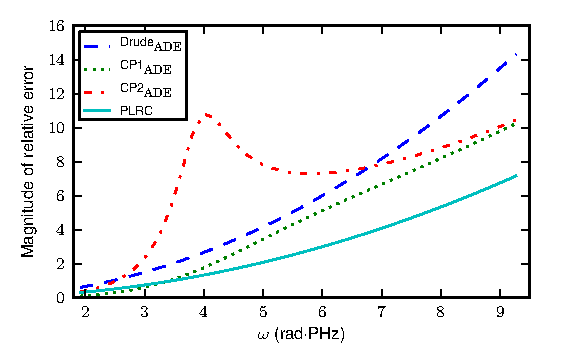
\includegraphics[width=0.45\textwidth]{figure/delta_gold}
      \label{fig:delta_gold}
    }
    \subfigure[silver]{
      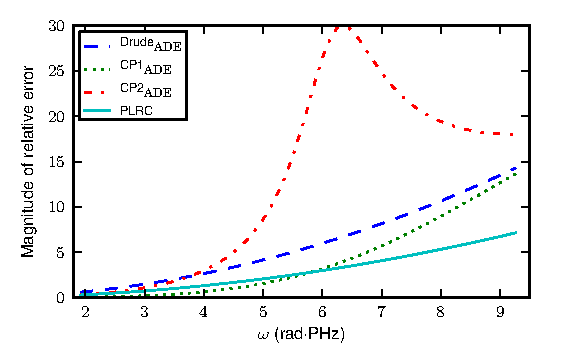
\includegraphics[width=0.45\textwidth]{figure/delta_silver}
      \label{fig:delta_silver}
    }
    \subfigure[copper]{
      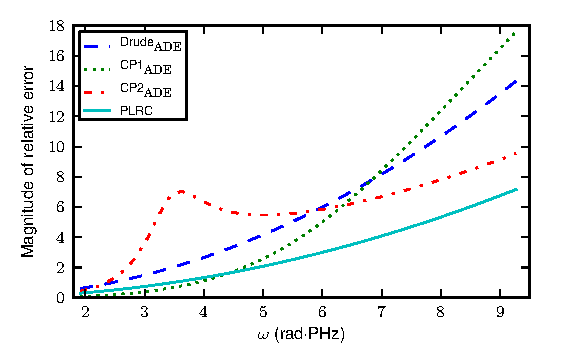
\includegraphics[width=0.45\textwidth]{figure/delta_copper}
      \label{fig:delta_copper}
    }
  \end{center}
  \caption{Frequency distribution of relative error of electric susceptibility magnitude from PLRC and ADE implementations of DCP model. CP1 and CP2 indicate the first and second critical points, respectively. For PLRC, the relative error for only one term is displayed since the relative errors of all terms are identical to each other. $\Delta t$ is set to 1 and the other parameters are listed in Table \ref{tab:dcp_param}.}
  \label{fig:delta_noble_metals}
\end{figure}

\section{Stability analysis}
Stability\index{stability} is one of the important criteria to be satisfied by the dispersive model when implemented into an FDTD algorithm. A stable system is a system where the errors that occur while solving the finite-difference equations of the FDTD scheme with dispersive models decay as time progresses, thereby not causing the simulation results to diverge.
  
The combination of the von Neumann method\index{von Neumann method} with the Routh-Hurwitz criterion\index{Routh-Hurwitz criterion} \cite{pereda_analyzing_2001} is used to derive the closed-form stability conditions for the FDTD representation of DCP media. As a result, the conditions that make Eq.~(\ref{eq:time_sampled_form}) stable for the Drude pole are
\begin{equation}
\begin{split}
s_1 \ge 0\\
s_2 \ge 0\\
s_2 s_3 - s_1 s_4 \ge 0\\
s_4 \ge 0
\end{split}
\end{equation}
and for a critical point are
\begin{equation}
\begin{split}
s_0 \ge 0\\
s_1 \ge 0\\
s_1 s_2 - s_0 s_3 \ge 0\\
s_1 s_2 s_3 -s_0 s_3^2 - s_1^2 s_4 \ge 0\\
s_4 \ge 0
\end{split}
\end{equation} 
where
\begin{equation}
\begin{split} 
s_0 = & \nu^2 \left( g_0 + g_1 + g_2 \right) \epsilon_\infty\\
s_1 = & 2 \nu^2 \left( -g_0 + g_2 \right) \epsilon_\infty\\
s_2 = & h_0 + h_1 + h_2 + \left( g_0 + \left( 1 - 2 \nu^2 \right) g_1 + g_2\right) \epsilon_\infty\\
s_3 = & -2 \left( h_0 - h_2 + \left( 1 - \nu^2 \right) \left( g_0 - g_2 \right) \epsilon_\infty \right)\\
s_4 = & h_0 - h_1 + h_2 + \left( 1 - \nu^2 \right) \left( g_0 - g_1 + g_2 \right) \epsilon_\infty.
\end{split}
\end{equation}
The parameter $\nu$ is defined as
\begin{equation}
\nu^2 = (c_\infty \Delta t)^2 \left ( \frac{\sin^2 \frac{\tilde{k}_x \Delta x}{2}}{\Delta x^2} + \frac{\sin^2 \frac{\tilde{k}_y \Delta y}{2}}{\Delta y^2} + \frac{\sin^2 \frac{\tilde{k}_z \Delta z}{2}}{\Delta z^2} \right )
\end{equation}
where $c_\infty = (\mu \epsilon_\infty \epsilon_0)^{-1/2}$, $\tilde k_{x,y,z}$ are the spatial components of the numerical wavevector, $\Delta x$, $\Delta y$ and $\Delta z$ are the spatial differences along x, y and z directions, respectively. 

The stability condition for the ADE implementation of the Drude pole is 
\begin{equation}
0 \le \nu^2 \le 1
\label{eq:non_dispersive_stable_cond}
\end{equation}
and is the same as the condition for the non-dispersive FDTD case. However, the PLRC implementation of the Drude pole has stricter condition to be satisfied,
\begin{equation}
0 \le \nu^2 \le 1 + \left[\frac{\omega _D^2}{\gamma^3 \Delta t \epsilon_\infty} \left( -\gamma  \Delta t + 2 \tanh \frac{\gamma \Delta t}{2} \right)\right].
\end{equation}
The terms inside the square brackets will always be negative, and hence the range of $\nu^2$ will be more restricted than Eq.~(\ref{eq:non_dispersive_stable_cond}). 

For the ADE implementation of the critical point, provided that the conditions
\begin{equation}
\sin \phi_p \le 0
\label{eq:ade_complementary_cond1}
\end{equation}
and
\begin{equation}
\left( \Gamma_p^2 - \Omega_p^2 \right) \sin \phi_p  \le 2 \Gamma_p \Omega_p \cos \phi_p
\label{eq:ade_complementary_cond2}
\end{equation}
are satisfied, the stability condition will be the same as that of the non-dispersive FDTD case.

\section{Fitting parameters for DCP model of noble metals}
A fitting procedure was performed to confirm the feasibility of our implementation of the DCP model in correctly representing the dielectric constants of noble metals. The parameters of noble metals were optimized by minimizing a fitness function $\Phi$ defined as
\begin{equation}
\Phi = \sum_\omega \left| \epsilon_\text{T}(\omega) - \epsilon(\omega)\right|^2
\end{equation}
where $\epsilon_T$ is tabulated values in the range from 200 to 1000 nm given in \citet{johnson_optical_1972}. We set all the parameters of the DCP model to have non-negative values except $\phi_p$, that was set in the range of $-\pi \le \phi_p \le 0$ to satisfy Eq.~(\ref{eq:ade_complementary_cond1}). The optimized parameters of the DCP model for noble metals are shown in Table \ref{tab:dcp_param}. Note that the parameters shown in Table \ref{tab:dcp_param} do not satisfy Eq.~(\ref{eq:ade_complementary_cond2}). We did not choose the optimized parameters that satisfy Eq.~(\ref{eq:ade_complementary_cond2}), because their fitness values are 1.2-4.5 times higher than that of the parameters in Table \ref{tab:dcp_param}. The real and imaginary values of relative electric permittivity obtained through fitting and experiments are plotted in figure \ref{fig:noble_metals_permittivity}. A good agreement is observed between the experimental value in \citet{johnson_optical_1972} and the DCP model for various noble metals with our optimized parameters.

\begin{table}[hp!]
  \centering 
  \begin{tabular}{lr@{.}lr@{.}lr@{.}l}
    \hline
    & \multicolumn{2}{c}{gold} & \multicolumn{2}{c}{silver} & \multicolumn{2}{c}{copper} \\
    \hline
    \hline
    $\epsilon_\infty$                             & 1&11683  & 0&89583   & 1&82307    \\
    $\omega_D$ ($\textrm{rad}\cdot\textrm{PHz}$) & 13&1839  & 13&8737   & 13&3846     \\
    $\gamma$ ($\textrm{rad}\cdot\textrm{PHz}$)   & 0&109173 & 0&0207332 & 0&163439    \\
    $A_1$                                        & 3&04155  & 1&3735    & 2&57278     \\
    $\phi_1$ ($\textrm{rad}$)                    & -1&09115 & -0&504659 & -1&56922e-8 \\
    $\Omega_1$ ($\textrm{rad}\cdot\textrm{PHz}$) & 4&20737  & 7&59914   & 6&65296     \\
    $\Gamma_1$ ($\textrm{rad}\cdot\textrm{PHz}$) & 2&35409  & 4&28431   & 3&80643     \\
    $A_2$                                        & 0&273221 & 0&304478  & 0&638294    \\
    $\phi_2$ ($\textrm{rad}$)                    & -1&18299 & -1&48944  & -1&22019    \\
    $\Omega_2$ ($\textrm{rad}\cdot\textrm{PHz}$) & 3&88123  & 6&15009   & 3&39199     \\
    $\Gamma_2$ ($\textrm{rad}\cdot\textrm{PHz}$) & 0&452005 & 0&659262  & 0&472389    \\
    \hline
    $\Phi$                                       & 3&6308   & 1&06454   & 6&07769     \\
    \hline
  \end{tabular}
  \caption{Parameters for the DCP model to fit the dielectric functions of noble metals over the $200<\lambda<1000~\textrm{nm}$ wavelength range (experimental data from \citet{johnson_optical_1972}). These parameters do not satisfy Eq.~(\ref{eq:ade_complementary_cond1}).}
  \label{tab:dcp_param}
\end{table}

\begin{figure}[hp!]
  \begin{center}
    \subfigure[Real part of the relative electric permittivity of noble metals]{
      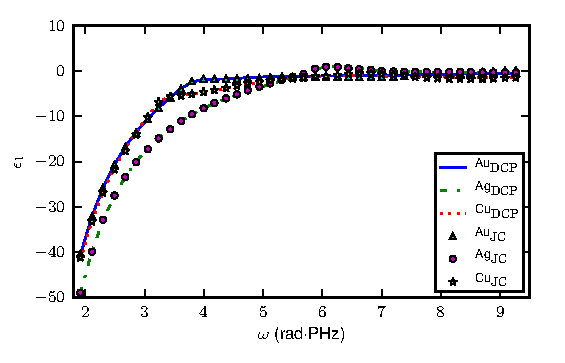
\includegraphics{figure/noble_metals_eps1}
      \label{fig:noble_metals_eps1}
    }
    \subfigure[Imaginary part of the relative electric permittivity of noble metals]{
      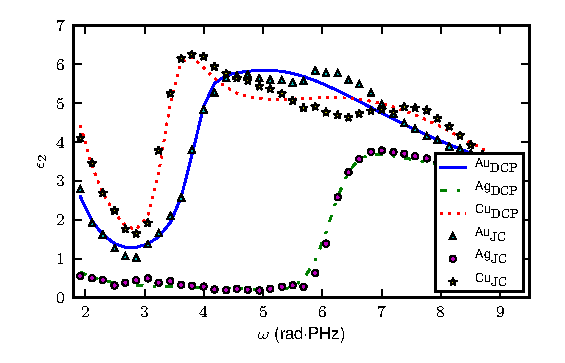
\includegraphics{figure/noble_metals_eps2}
      \label{fig:noble_metals_eps2}
    }
  \end{center}
  \caption{Permittivity of noble metals and its description using DCP model. The label with JC in the subscript means that the data comes from \citet{johnson_optical_1972}.}
  \label{fig:noble_metals_permittivity}
\end{figure}

\section{Numerical experiments}
The PLRC and ADE schemes for the DCP model have been implemented using an inhouse-developed FDTD package called GMES\footnote{http://sourceforge.net/projects/gmes}. The validation of our implementation was done by performing numerical experiments in which the transmission and reflection of light by a thin metal film was studied. Using the parameters given in Table \ref{tab:dcp_param}, we computed the transmittance and reflectance of light through a thin film made of noble metals surrounded by air as a function of the incident light frequency. A continuous wave source was used as excitation, and the simulations were performed in 1-dimensional space with light incident normally on the metal films made of gold, silver, and copper. The FDTD parameters are $\Delta x=1~\text{nm}$, $\Delta t=\Delta x/(2c)$ where $c$ is the speed of light in vacuum. The numerical results were compared to the results from the analytical method \cite{born_principles_1999}. As shown in figure \ref{fig:thin_metals_t_r}, an excellent agreement is observed between the numerical and analytic results for all the metals and implementation schemes considered  (ADE and PLRC), which validates our implementation schemes.

\begin{figure}[hp!]
  \begin{center}
    \subfigure[gold]{
      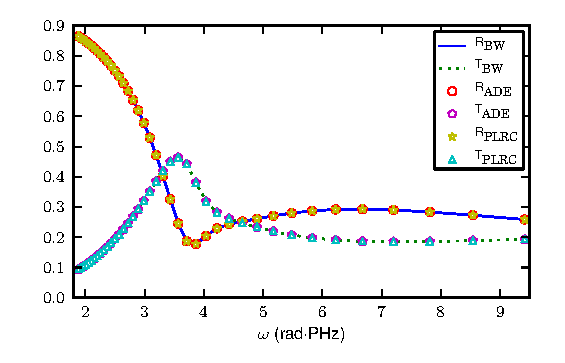
\includegraphics[width=0.45\textwidth]{figure/au_t_r}
      \label{fig:thin_au_t_r}
    }
    \subfigure[silver]{
      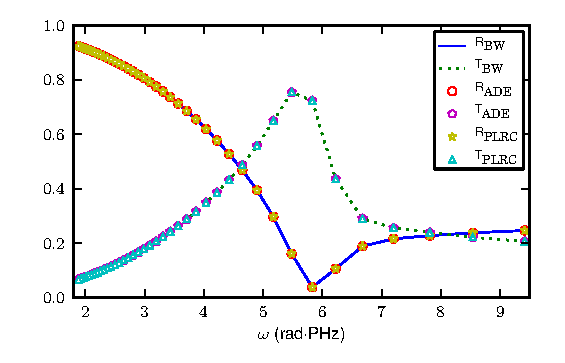
\includegraphics[width=0.45\textwidth]{figure/ag_t_r}
      \label{fig:thin_ag_t_r}
    }
    \subfigure[copper]{
      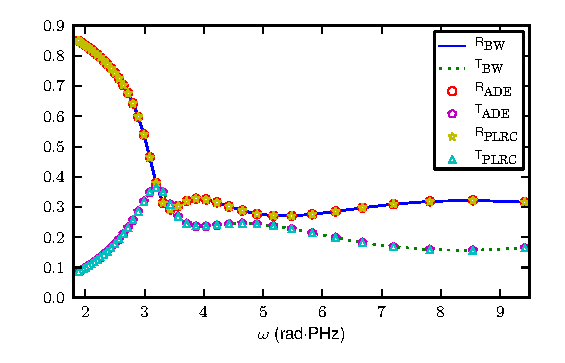
\includegraphics[width=0.45\textwidth]{figure/cu_t_r}
      \label{fig:thin_cu_t_r}
    }
  \end{center}
  \caption{Transmittance and reflectance of the normal incidence of light through a thin metal film. BW in the label indicates the analytical results from \citet{born_principles_1999}.}
  \label{fig:thin_metals_t_r}
\end{figure}

In order to further compare the implemented schemes, magnitude of the relative errors for various implementations are plotted in figure \ref{fig:thin_metals_t_r_error} for the case of gold, silver, and copper. In this case, apart from the ADE and PLRC schemes, the comparison was done for RC scheme by setting the $\xi$ related terms to 0 as discussed in Section \ref{sec:impl_plrc}. As seen from figure \ref{fig:thin_metals_t_r_error}, the relative error for reflectance and transmittance of the ADE and PLRC schemes are much lower compared to that of RC scheme for all the metals, except in the case of gold where the RC scheme shows lower errors for transmittance for frequencies above 5 rad$\cdot$PHz. It is observed that the maximum error of reflectance and transmittance from ADE and PLRC implementations are less than 0.066 \% which are much lower than that from RC implementation (0.433 \%).

\begin{figure}[hp!]
  \begin{center}
    \subfigure[gold]{
      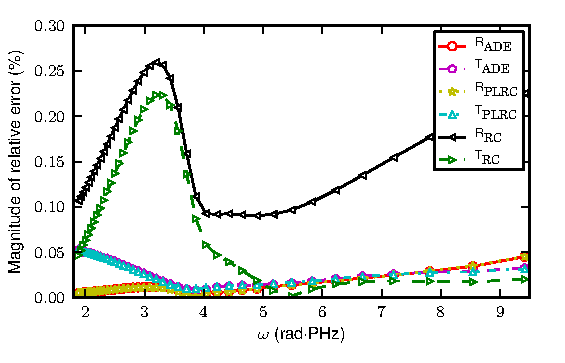
\includegraphics[width=0.45\textwidth]{figure/au_t_r_error}
      \label{fig:thin_au_t_r_error}
    }
    \subfigure[silver]{
      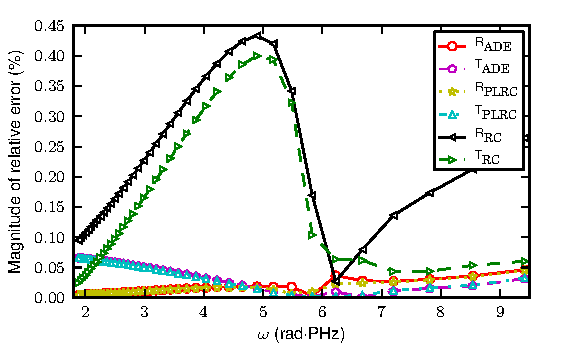
\includegraphics[width=0.45\textwidth]{figure/ag_t_r_error}
      \label{fig:thin_ag_t_r_error}
    }
    \subfigure[copper]{
      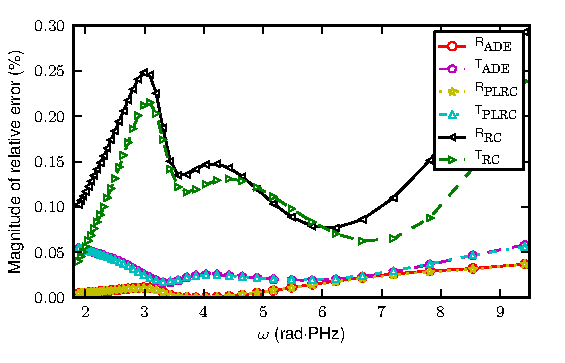
\includegraphics[width=0.45\textwidth]{figure/cu_t_r_error}
      \label{fig:thin_cu_t_r_error}
    }
  \end{center}
  \caption{Relative error of transmittance and reflectance through a thin metal film for various metals in ADE, PLRC, and RC schemes.}
  \label{fig:thin_metals_t_r_error}
\end{figure}

\section{Conclusions}
We have shown the implementation of DCP model for describing dispersive media using PLRC and ADE schemes into FDTD algorithm. It was shown that DCP model can correctly describe the experimentally reported permittivity values of various metals. Comparison of PLRC and ADE implementations showed that PLRC scheme requires lesser memory, while ADE scheme requires only fewer arithmetic operations. It was found that the numerical error of the PLRC implementation was less compared to that of ADE implementation for the metals considered. Stability analysis of both schemes showed that ADE scheme can have the same stability condition to that of the non-dispersive FDTD case. Finally, the implementation schemes were applied in studying the transmittance and reflectance of thin metal films, and excellent agreement was observed between the analytical and numerical results, thus validating our implementations.  
